%\documentclass[10pt,a4paper,twocolumn,draft]{article}
\documentclass[10pt,a4paper]{article}
\usepackage[utf8]{inputenc}
\usepackage[ngerman]{babel}
\usepackage{amsmath}
\usepackage{amsfonts}
\usepackage{amssymb}
\usepackage{algorithm}
\usepackage[noend]{algpseudocode}
\usepackage{url}
\usepackage{hyperref}
\usepackage{graphicx}


\begin{document}
\author{Gruppe 2}
\title{Portierung und Parallelisierung mehrerer Filter von GIMP nach GEGL}
\maketitle

\section*{Abstract}

% works with: \usepackage{algorithm} AND \usepackage[noend]{algpseudocode}
% works with: \usepackage{graphicx}
\part{Glass Tile}

\section{Einleitung}
 
\subsection{Beschreibung des Filters aus Nutzersicht}
Dieses Filter lässt das Bild erscheinen, als würde es durch eine Wand aus Glasbausteinen betrachtet werden. Das Filter kann auf die aktive Ebene oder eine im Bild befindliche Auswahl angewendet werden.\footnote{\url{http://docs.gimp.org/de/plug-in-glasstile.html}} Die Kachelbreite und Kachelhöhe sind individuell einstellbar.
\subsection{Algorithmus} 
%Pseudocode, visuell
\begin{algorithm}[h]
\caption{Pseudo-Code des \glqq Glass Tile\grqq-Algorithmus}
\label{algo:gtile}
\begin{algorithmic}[1]
\State $xhalf = tileWidth  / 2$
\State $yhalf = tileHeight / 2$
\State $xplus = tileWidth  \mod 2$
\State $yplus = tileHeight \mod 2$
\State $ymiddle = yoffs = 0$
\ForAll{$rows$ $r$ $\in input$}
	\State $ypixel2 = ymiddle + yoffs * 2$
	\State lese Zeile $ypixel2$ aus dem Eingabebild
	\State $yoffs$++
	\If{$yoffs == yhalf$}
		\State{$ymiddle = ymiddle + tileHeight$}
		\State{$yoffs = - (yhalf + yplus)$}
	\EndIf
	\State $xmiddle = xoffs = 0$
	\ForAll{$columns \in column$}
		\State $xpixel1 = (xmiddle + xoffs)$
		\State $xpixel2 = (xmiddle + xoffs * 2)$
		\State schreibe Pixel $xpixel2$ aus Eingabezeile nach $xpixel1$ in Ausgabezeile
		\State $xoffs$++
		\If{$xoffs == xhalf$}
			\State{$xmiddle = xmiddle + tileWidth$}
			\State{$xoffs = - (xhalf + xplus)$}
		\EndIf
	\EndFor
	\State speichere Ausgabezeile an Zeilenposition $r$ im Ausgabebild
\EndFor	
\end{algorithmic}
\end{algorithm}

%Beschreibung Algorithmus allgemeinsprachlich
Der Algorithmus erzeugt sowohl zeilenweise als auch spaltenweise eine Verrückung und Wiederholung innerhalb der Kacheln. Dabei wird jede zweite Zeile in einer Kachel hintereinander in die erste Hälfte der Kachel verschoben wie in Abbildung~\ref{fig:gtile1} zu sehen.
\begin{figure}[h]
\begin{center}
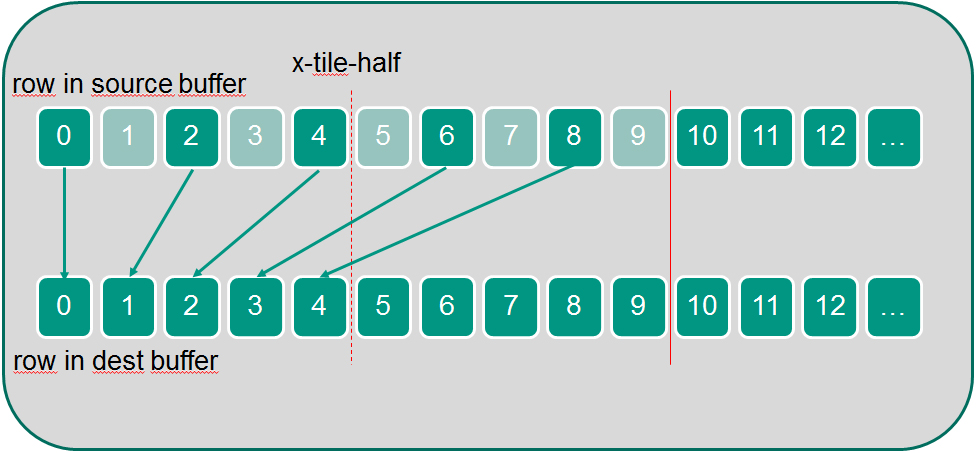
\includegraphics[scale=.4]{gtile1.png}
\end{center}
\caption{Verrückung der Spalten innerhalb einer Zeile}\label{fig:gtile1}
\end{figure}
Diese gelesenen und verschobenen Zeilen werden anschließend in der zweiten Hälfte nochmals wiederholt, was in Abbildung~\ref{fig:gtile2} dargestellt ist.
\begin{figure}
\begin{center}
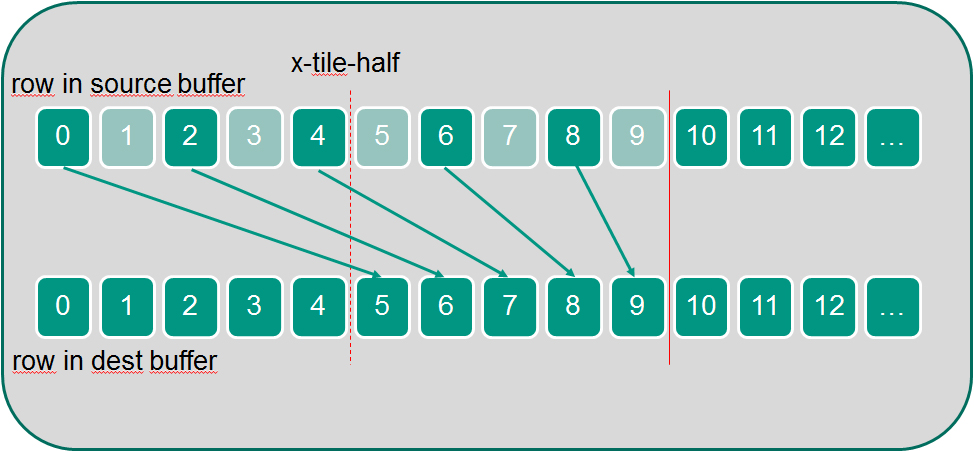
\includegraphics[scale=.4]{gtile2.png}
\end{center}
\caption{Wiederholung der verrückten Spalten innerhalb einer Kachelzeile}\label{fig:gtile2}
\end{figure}
Die Verrückung und Wiederholung der Spalten erfolgt analog. Auf diese Weise wird Kachel für Kachel bearbeitet. Der sequentielle original Algorithmus liest dabei komplette Zeilen ein und führt darauf die notwendigen Spaltenverschiebungen durch.

\subsection{Zielsetzung}
%Portierung von GIMP nach GEGL
%Parallelisierung mittels OpenMP
\section{Portierung}
%Beibehaltung der Farbrepräsentation in RGBA u8
%Beibehaltung bereits in GIMP vorhandener Bug 

\section{Parallelisierung}
\section{Auswertung}

\subsection{Korrektheit}
 
%Bild Eingabe (Duck / matting-global / car-stack?)
%Vergleich Ausgabe bei Eingabe mit gleichen Parametern GIMP – GEGL Bilder
%Ergebnis vom Diff
\subsection{Laufzeit}
 
%X Durchläufe in Diagram abtragen?
%System beschreiben (Hardware, Software, Umgebungsvariablen) !!!
%Boxplots !!!
%Statistische Analyse ?!
%Aus Debug-Output Diagramm erstellen um Anteil des Filters an Gesamtlaufzeit zu verdeutlichen
\section{Evaluation der Ergebnisse}

%Warum wird es mit OpenMP langsamer?
\section{Ausblick}
%Umstellung auf Floats
%Behebung des Bugs
%Implementierung in OpenCL
\end{document}